\documentclass[11pt,a4paper]{article}
\usepackage[utf8]{inputenc}
\usepackage[T1]{fontenc}
\usepackage{tikz}
\usepackage{amsmath,amsfonts,amssymb,amsthm}
\usepackage{graphicx}
\usepackage{mathtools}
\usepackage[lastexercise]{exercise}
\usepackage{fullpage}


\title{TD2 MVFA: Linear-Time properties} %chktex 13
\date{}

\renewcommand{\ExerciseHeader}{\textbf{\Large\ExerciseName\ \ExerciseHeaderNB\ExerciseHeaderTitle\ExerciseHeaderOrigin\medskip}}
\renewcommand{\AnswerHeader}{\bigskip\textbf{Answer of exercise \ExerciseHeaderNB}\medskip}


\def\exercise#1{\Large\textbf{Exercise #1}\normalsize\\}
\def\question#1{\textbf{Question #1:}\quad}

\def\ts{\mathcal{TS}}
\def\tss{\mathcal{TS^*}}
\def\traces{\mathit{Traces}}
\def\seta{\{a\}}
\def\setab{\{a,b\}}

\newcommand\badp{\mathit{BadPref}}
\newcommand\pref{\mathit{Pref}}
\newcommand\twoap{2^{AP}}
\renewcommand\star{^*}
\newcommand\cl{\mathit{Cl}}

\newtheorem*{lemma}{Lemma}
\newtheorem*{theorem}{Theorem}
\DeclareMathOperator{\Pref}{Pref}
\DeclareMathOperator{\Cl}{Cl}

\begin{document}
\maketitle

\begin{Exercise}

Give the traces on the set of atomic propositions $\{a,b\}$ of the following transition system:

\begin{center}
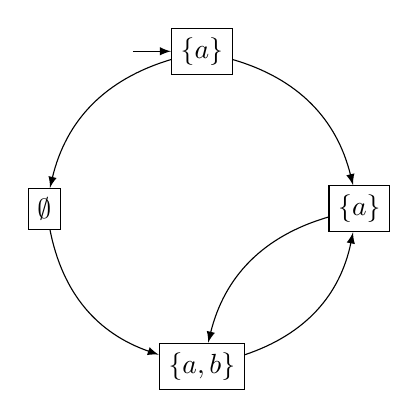
\begin{tikzpicture}
\node[draw] (s0) at (0,0) {$\emptyset$};
\node[draw] (s1) at (2,-2) {$\{a,b\}$};
\node[draw] (s2) at (2,2) {$\{a\}$};
\node[draw] (s3) at (4,0) {$\{a\}$};
\node (i) at (1,2) {};
\draw[-latex] (s0) [bend right] to (s1);
\draw[-latex] (s1) [bend right] to (s3);
\draw[-latex] (s3) [bend right] to (s1);
\draw[-latex] (s2) [bend right] to (s0);
\draw[-latex] (s2) [bend left] to (s3);
\draw[-latex] (i) -- (s2);
\end{tikzpicture}
\end{center}
\end{Exercise}

\begin{Answer}

Let $\ts$ be the transition system. There is only two possibles executions in $\ts$, with distinct traces.% I don't understand this sentence -> a 2 was missing
We have:
$$\traces(\ts)=\seta{(\seta\setab)}^\omega\ +\ \seta\emptyset{(\setab\seta)}^\omega$$
\end{Answer}

\begin{Exercise}

You have seen a way to transform a transition system $TS$ with terminal states into an ``equivalent'' transition system $TS^*$ without terminal states.

\begin{enumerate}
	\item Give a formal definition of this transformation.
	\item Prove that the transformation preserves trace-equivalence, \textit{i.e.} show that if $TS_1$ and $TS_2$ are such that $Traces(T_1) = Traces(T_2)$, then $Traces(T_1^*) = Traces(T_2^*)$.
\end{enumerate}
\end{Exercise}

\begin{Answer}
\Question%
Let $\ts=(S,\mathit{Act},\rightarrow,S_0,\mathit{AP},L)$ be a transition system.

We define another transition system without terminal states, $\tss$. Informally, it corresponds to $\ts$ without terminal states: each terminal state has been redirected to a new state which loops on itself.

We define $\ts^*$ with:

$$\tss=(S\uplus\{\Omega\},\mathit{Act}\uplus\{\alpha\},\rightarrow^*,S_0,\mathit{AP},L^*)$$

in which:
\begin{itemize}
	\item $\Omega$ is a new state and $\alpha$ a new action;
	\item $\rightarrow^*$ is defined by:
		$$\rightarrow^*\quad=\quad\rightarrow\quad\cup\quad\{v\xrightarrow{\alpha} \Omega~|~\nexists (s\in S, \beta\in\mathit{AP}), v\xrightarrow{\beta}s\}\quad\cup\quad\{\Omega\xrightarrow{\alpha}\Omega\}$$% there does not exist --> for all? Moreover, there's a problem with the spacing in this formula, I'll see if I can fix it later
		This means that every pair of connected states in $\mathcal{TS}$ is still a pair of connected states in $\mathcal{TS^*}$, any state with no successor is connected to $\Omega$. Finally, $\Omega$ is connected to itself.
	\item $L^* : S\uplus\{\Omega\} \to \mathit{AP}$ is such that $\forall s\in S,  L^*(s) = L(s)$ and $L^*(\Omega) = \emptyset$.
\end{itemize}

Note that with this construction, we do not have the other implication. %equivalence of trace-equivalence in $\ts$ and $\tss$, as this last adds new path ending with $\emptyset^\omega$.
It is not necessary in our context if we just want to answer the question. %, as we only want the first implication. %If this refinement is nevertheless wanted, it can be obtained by defining a new proposition true only in state $\Omega$.

More formally, there exists some $\ts_1$ and $\ts_2$ such that $\traces(\tss_1)=\traces(\tss_2)$ but $\traces(\ts_1)\neq\traces(\ts_2)$. This implication was not to be proven. However, if we really wanted that equivalence, we could change $L^*$ such that $L^*(\Omega)=\text{STOP}$ where $\text{STOP}$ is a new property. Defining it with $\emptyset$ is easier to understand. % is it better now?

% I don't understand. Does this mean that the reverse transformation does not preserve trace-equivalence?
% If this is the case, there is two problems: 1/ it is not clear that we can define such a reverse transformation
% 2/ even if this is the case, it is not obvious that it would not preserve trace-equivalence. need an example.
% An example could be as follow: consider the ts 1 -> 2 -> 3 with L(1) = L(1) = {A} and L(3) = \emptyset, and the same with a loop on 3. The resulting non halting ts would both have a language of trace of {A}{A}(\emptyset)^\omega. Yet the trace languages of the 2 original ts are different.	

\Question%
We introduce a lemma that will be helpful in order to prove the theorem.
\begin{lemma}
  \begin{align*}
    \traces(\tss) &= \{t\in\traces(\ts) \mid t\text{ is infinite}\}\\
    &\cup\{t\emptyset^\omega \mid t\in\traces(\ts)\text{ and $t$ is finite}\}
  \end{align*}
\end{lemma}
\begin{proof}
  By double inclusion.\\
  \begin{itemize}
	  \item \reflectbox{$\subseteq$}: % explain more? -> Proof proposal
	  \begin{itemize}
		  \item Let $t\in \traces(\ts)$ be the infinite trace of execution $e$. As $t$ is infinite, so is $e$ (there is a state in $e$ for each subset of $AP$ in $t$).
		  Then $e$ never reaches a terminal state, else it would not be infinite. So $e\in \traces(\tss)$ as $\tss$ is equal to $\ts$ out of the terminal states and $\Omega$.
		  \item Let $t\in \traces(\ts)$ be a finite trace corresponding to a finite execution $e$. Then $e$ ends in a terminal state. Thus, $e$ is an execution fragment over $\tss$
		  (by construction of $\tss$, all execution fragments over $\ts$ fit $\tss$). Let $s$ be the final state in which $e$ ends. There is no execution fragment in $\ts$ starting in $s$ as it is a terminal state.
		  Hence in $\tss$, only $\emptyset^\omega$ starts in $s$, corresponding to the execution $s\Omega^\omega$. The concatenation of these two fragments (which is a complete execution in $\tss$) is possible in $\tss$ and has for trace $t\emptyset^\omega$.
	  \end{itemize}
	  \item $\subseteq$: Here it is easier to work directly with the underlying execution.
	  Let $t\in \traces(\tss)$ be the trace of execution $e$. Let us discuss on whether the execution reaches $\Omega$ or not.
	  \begin{itemize}
		  \item If $e$ reaches $\Omega$ at some point, then as $Post(\Omega) = \{\Omega\}$, $e=e'\Omega^\omega$ where $e'$ is a finite (and initial) execution fragment without $\Omega$ over $\tss$.
		  So $e'$ is an initial finite execution fragment over $\ts$. Furthermore the last state $s$ of $e$ is such that $\Omega \in Post(s_{\tss})$, so by construction of $\tss$, $Post(s_{\tss})=\Omega$ and
		  $Post(s_{\ts})=\emptyset$. Hence $e'$ is maximal, i.e. $e'$ is a finite execution of $\ts$ of trace $t'$. By construction of $e$ and $t$ (the initial trace over $\tss$), $t = t'\emptyset^\omega$.
		  \item If $e$ does not reach $\Omega$, then $e$ is an infinite execution over $\ts$ and $t\in  \{t\in\traces(\ts)~|~t\text{ is infinite}\}$.
	  \end{itemize}
  \end{itemize}
\end{proof}


\begin{proof}[Trace-equivalence preservation] We can now prove the theorem, by double inclusion.

Let $\ts_1$ and $\ts_2$ be two transition systems such that $\traces(\ts_1)=\traces(\ts_2)$. Let $t_1\in\traces(\tss_1)$. Let us show that $t_1\in\traces(\tss_2)$.

According to the previous lemma, $t_1$ can either be in $\{t\in\traces(\ts_1)~|~t\text{ is infinite}\}$ or in $\{t\ \emptyset^\omega~|~t\in\traces(\ts_1)\text{ and $t$ is finite}\}$.

If $t_1\in\{t\in\traces(\ts_1)~|~t\text{ is infinite}\}$, then $t_1\in\traces(\ts_1)=\traces(\ts_2)$. Thus, $t_1$ is an infinite trace of $\ts_2$ and then by the previous lemma, $t_1\in\traces(\tss_2)$.

If $t_1\in\{t\ \emptyset^\omega~|~t\in\traces(\ts_1)\text{ and $t$ is finite}\}$, then $t_1=t\ \emptyset^\omega$ where $t$ is a finite trace of $\ts_1$ and thus a finite trace of $\ts_2$ as well. Then by the previous lemma, $t\ \emptyset^\omega$ is also a trace of $\tss_2$.

We thus have that every trace of $\tss_1$ is a trace of $\tss_2$, which means $\traces(\tss_1)\subseteq\traces(\tss_2)$. The other inclusion is symmetric. We thus have proved that, whenever $\traces(\ts_1)=\traces(\ts_2)$, $\traces(\tss_1)=\traces(\tss_2)$.
\end{proof}
\end{Answer}

\begin{Exercise}

Consider the set $AP$ of atomic propositions defined by $AP = \{ x = 0,x > 0 \}$ and consider a non-terminating sequential computer program $P$ that manipulates the variable $x$.

Formulate the following informally stated properties as LT properties:
\begin{enumerate}
\item false;
\item initially $x$ is equal to zero;
\item initially $x$ differs from zero;
\item initially $x$ is equal to zero, but at some point $x$ exceeds zero;
\item $x$ exceeds zero only finitely many times;
\item $x$ exceeds zero infinitely often;
\item the value of $x$ alternates between zero and not zero;
\item true.
\end{enumerate}

Determine which of the provided LT properties are
safety properties and which are liveness properties.
\end{Exercise}

\begin{Answer}

% Why does \badp have parenthesis and not \pref?

We name the properties $P_1, P_2\dots P_8$.
Recall the definition of safety property and liveness property:
\begin{itemize}
	\item $E$ is called a \emph{safety property} if for all words
		$$\sigma = A_0A_1A_2\dots\in{(\twoap)}^\omega\setminus E$$
		there exists a finite prefix $A_0A_1\dots A_n$ of $\sigma$ such that none of the words $$A_0A_1\dots A_nB_{n+1}B_{n+2}\dots$$ belongs to E. %chktex 25
	\item $E$ is called a \emph{liveness property} if each finite word can be extended to an infinite word in $E$, ie.\ $\pref(E) = {(\twoap)}^+$.
\end{itemize}
  \Question%
  $P_1 = \emptyset$\\
Every prefix is a bad prefix for the property \textit{false}, because the property is always false. Thus, $\badp(P_1) = (\twoap)\star$ and $\pref{P_1} = \emptyset$. As $\pref(P_1)\neq (\twoap)\star$, the property is not a liveness property. However, the property is a safety property. Indeed, for each infinite word $\Omega$, there exists a finite prefix that cannot be extended into a word that satisfies the property: any prefix of $\Omega$ is such a prefix. %this sentence is too long. Maybe we could recall the definition of safety property at the beginning of the exercise.
% Moreover, it is for each infinite word that doesn't satisfy the property. here is it the same, but mb it could be made clearer.
% Why not replace the last sentence by $\badp(P_1) = (\twoap)\star = (\twoap)\star\\ \emptyset, which is the definition of safety property?$
  \Question%
  $P_2 = \{x = 0\}(\twoap)^\omega$\\
For such a property, one can define a set of bad prefixes: $\badp(P_2) = \{x > 0\}(\twoap)\star$. Any infinite word that make the property false has such a bad prefix. Thus, the property is a safety property. However, since $\badp(P_2)\neq\emptyset$, there exists some finite words that cannot be extended into an infinite word that satisfies the property. Thus, the property is not a liveness property.
  \Question%
  $P_3 =  \{x > 0\}(\twoap)^\omega$\\
This property is also a safety property, with $\badp(P_3) = \{x=0\}(\twoap)\star$. It isn't a liveness property because the set of bad prefixes isn't empty.
  \Question%
  $P_4 = \{x = 0\}(\twoap)\star\{x > 0\}(\twoap)^\omega$\\
This property isn't a liveness property: for instance, the finite prefix $\{x>0\}$ cannot be extended to an infinite word that satisfies the property.
This property isn't a safety property either. Indeed, we have that the word ${\{x=0\}}^\omega\in\cl(P_4)$ but ${\{x=0\}}^\omega\not\in P_4$. And we know that a property $E$ is a safety property iff $\cl(E)=E$.
  \Question%
  $P_5 = ((\twoap)\star\{x > 0\})\star(\{\{x=0\},\emptyset\})^\omega$\\  
The property is a liveness property, because the set of good prefixes $\pref(P_5)$ is equal to $(\twoap)\star$, because  every finite word can be extended into a infinite word in which zero is exceeded only finitely many times. This property isn't a safety property, because ${\{x>0\}}^\omega\in\cl(P_5)-P_5$ and thus $\cl(P_5)\neq P_5$.
% isn't it x>0 ? 
  \Question%
  $P_6 = ((\twoap)\star\{x > 0\})^\omega$\\
$P_6$ is a liveness property. Indeed, let $\sigma$ be a finite word. One can extend $\sigma$ such that the result exceeds zero infinitely often. For instance, consider the infinite word ${\sigma(\{x>0\})}^\omega$.
However, $P_6$ isn't a safety property: ${\{x=0\}}^\omega\in\cl(P_6)-P_6$ and thus $\cl(P_6)\neq P_6$.
  \Question%
  $P_7 = (\{x = 0\}\{x > 0\})^\omega + (\{x > 0\}\{x = 0\})^\omega$\\
$P_7$ is a safety property because we can characterize it with its set of bad prefixes: $\badp(P_7)=(\twoap)\star\ (\{x=0\}\{x=0\} + \{x>0\}\{x>0\}) (\twoap)\star$. Indeed, every infinite word that does not satisfy the property contains either $\{x=0\}\{x=0\}$ or $\{x>0\}\{x>0\}$.
However, $P_7$ is not a liveness property, $\{x=0\}\{x=0\}$ is a word that cannot be extended to an infinite word that satisfies $P_7$.
  \Question%
  $P_8 = (\twoap)^\omega$\\
$P_8$ is both a safety and liveness property. We can describe its bad prefixes: $\badp(P_8)=\emptyset$. And since this set is empty, every finite prefix can be extended to a infinite word of $P_8$, since every infinite word is a word of $P_8$.
\end{Answer}

\begin{Exercise}

Let $P$ and $P'$ be two LT properties. Prove or disprove: $Pref(P) = Pref(P')$ if and only if $Cl(P) = Cl(P')$.
\end{Exercise}

\begin{Answer}

  Let $P$ and $P'$ be two LT properties. Let us show that the following theorem is true:
  \begin{theorem}
    $\Pref(P) = \Pref(P')$ if and only if $\Cl(P) = \Cl(P')$
  \end{theorem}
  \begin{proof}
    We prove the two implications.
    \begin{description}
      \item[($\Rightarrow$)]
        Suppose $\Pref(P) = \Pref(P')$. We have:
        \begin{align*}
          \Cl(P) &= \{\sigma\in{(2^{\textrm{AP}})}^\omega \mid \Pref(\sigma)\subseteq\Pref(P)\}\\
          &= \{\sigma\in{(2^{\textrm{AP}})}^\omega \mid \Pref(\sigma)\subseteq\Pref(P')\} &&\text{ since }\Pref(P) = \Pref(P')\\
          &= \Cl(P')&&\text{ (definition of closure)}
        \end{align*}
      \item[($\Leftarrow$)]
        Suppose $\Cl(P) = \Cl(P')$. We have two cases:
        \begin{description}
          \item[Case 1] One of $\Pref(P)$ or $\Pref(P')$ is empty.\\
          Suppose for example that $\Pref(P) = \emptyset$ Then $\Cl(P) = \emptyset = \Cl(P')$.\\
          Thus $\Pref(P') = \emptyset = \Pref(P)$.
          \item[Case 2] $\Pref(P) \neq \emptyset$
          Let $\sigma\in\Pref(P)$ be a prefix of $P$. \\
          There exists an (infinite) trace $\hat{\sigma} \in P$ such that $\sigma\in\Pref(\hat{\sigma})$.

          Since $\hat{\sigma}\in P\subset\Cl(P)$, we have that $\hat{\sigma}\in\Cl(P')$. \\
          Therefore $\sigma\in\Pref(P')$.\\
          $\Pref(P)\subseteq\Pref(P')$. The other inclusion is true for the same reason.

        \end{description}
    \end{description}
  \end{proof}
\end{Answer}

\begin{Exercise}
Let $P$ and $P'$ be liveness properties over $AP$. Prove or disprove the following claims:
\begin{enumerate}
\item $P \cup P'$ is a liveness property;
\item $P \cap P'$ is a liveness property.
\end{enumerate}
Answer the same questions for $P$ and $P'$ being safety properties.
\end{Exercise}

\begin{Answer}
\Question%
Let us prove that for $P$ and $P'$ two liveness properties, $P \cup P'$ is a liveness property.
\begin{align*}Pref(P \cup P') &= Pref(P) \cup Pref(P')\footnotemark[1]\\
                              &= {(2^{AP})}^* \cup {(2^{AP})}^* \text{ [P and P' are liveness properties]}\\
                              &= {(2^{AP})}^*
\end{align*}
So $P \cup P'$ is a liveness property.
\footnotetext[1]{If this equality is not known, we can convince ourselves by considering that being a prefix of a language by definition being a prefix of a given word,
and the words of $A\cup B$ are exactly the words of $A$ plus the words of $B$.}
\Question%
Let us show a counterexample proving that the intersection of two liveness properties is not always a liveness property.
Using the two liveness properties defined in exercise 3: $x$ exceeds zero only finitely many times; $x$ exceeds zero infinitely often.
The intersection of these two properties is $false$ which is not a liveness property (cf.\ exercise 3 again).
\Question%
Given $P$ and $P'$ two safety properties, we prove that $P\cup P'$ is a safety property, by using the definition of a safety property. Let $\sigma \in (\twoap)^\omega \setminus (P\cup P')$. Especially, $\sigma \in (\twoap)^\omega \setminus P$ and $\sigma \in (\twoap)^\omega \setminus P'$. Hence $\sigma \notin P$ and $\sigma \notin P'$, and as these are safety properties, no prefix of $\sigma$ can be completed in words of $P$ or $P'$. Thus no prefix of $\sigma$ can be completed in a word of $P \cup P'$ and $P \cup P'$ is a safety property. 
Formally: $$P\cap(\bigcup_{\gamma\quad prefix~of~\sigma} \{\alpha ~|~ \gamma \text{ can be completed in }\alpha \})=\emptyset$$ and $$P'\cap(\bigcup_{\gamma\quad prefix~of~\sigma} \{\alpha ~|~ \gamma \text{ can be completed in }\alpha \})=\emptyset$$ so $$(P\cup P')\cap(\bigcup_{\gamma\quad prefix~of~\sigma} \{\alpha ~|~ \gamma \text{ can be completed in }\alpha \})=\emptyset.$$ By definition, it comes that $P\cup P'$ is a safety property.

% Given $P$ and $P'$ two safety properties, we prove that $P\cup P'$ is a safety property, by reasoning on the bad prefixes. We show by double inclusion that $ (\twoap)^\omega \setminus (P\cup P')  = BadPref( P\cup P')$.
% \begin{itemize}
% \item $\alpha \notin P\cup P'$ implies $\alpha \notin P$ or $\alpha \notin P'$.
% For the simplicity of the notations, we will assume $\alpha \notin P$ is verified. Then $\alpha \in BadPref(P)$, i.e. $Pref(\alpha) \subseteq Pref(P) \subseteq Pref(P \cup P')$ and $\alpha \in BadPref(P \cup P')$.
% \item $\alpha \in BadPref(P\cup P')$ means $Pref(\alpha) \subseteq Pref(P \cup P')$ which implies $alpha \in BadPref(P)$ (or the same thing for $P'$, an the proof is symmetric). Then, by definition $\alpha \in P \subseteq (P \cup P')$.
% \end{itemize}
\Question%
Given $P$ and $P'$ two safety properties, we prove that $P\cap P'$ is a safety property, by showing the equality of this language with its closure.
As for any property $p$, $p \subseteq \Cl(p)$, we will prove the other inclusion. Lets consider $\alpha \in \Cl(P\cap P')$. By definition, $Pref(\alpha) \subseteq Pref(P\cap P') \subseteq Pref(P) \cap Pref(P')$ \footnotemark[2].
Specifically, $Pref(\alpha) \subseteq Pref(P)$, hence $\alpha \in \Cl(P) = P$. The same proof leads to $\alpha \in P'$. Hence $\alpha \in P\cap P'$.


\footnotetext[2]{As previously, if this is not known, convince yourself with this argument: being a prefix of $A\cap B$ is being the prefix of a word of $A \cap B$ which is a word of both $A$ and $B$.}
\end{Answer}


\end{document}
